\documentclass{article}

\usepackage[top=4cm,bottom=1.5cm,left=1.5cm,right=1.5cm]{geometry}
\usepackage{tikz}
\usetikzlibrary{calc}
\usetikzlibrary{positioning}
\usepackage{fancyhdr}
\usepackage{graphicx}
\usepackage{DejaVuSerifCondensed}
\usepackage[T1]{fontenc}
\usepackage{booktabs}
\usepackage{tabularx}
\usepackage{adjustbox}

\usepackage{titlesec}

\titleformat*{\paragraph}{\large\bfseries}
\titlespacing{\paragraph}{%
  0pt}{%              left margin
  0pt}{% space before (vertical)
  1em}%               space after (horizontal)


\newcommand{\titleframe}{%
\begin{tikzpicture}[remember picture, overlay]
    \node (A) [xshift=1.25cm,yshift=1.25cm] at (current page.south west) {};
    \node (B) [xshift=1.25cm,yshift=-1.25cm] at (current page.north west) {};
    \node (C) [xshift=-1.25cm,yshift=-1.25cm] at (current page.north east) {};
    \node (D) [xshift=-1.25cm,yshift=1.25cm] at (current page.south east) {};

    \coordinate (cA) at (A);
    \coordinate (cB) at (B);
    \coordinate (cC) at (C);
    \coordinate (cD) at (D);

    \coordinate[xshift=1mm, yshift=1mm] (dA) at (A);
    \coordinate[xshift=1mm, yshift=-1mm] (dB) at (B);
    \coordinate[xshift=-1mm, yshift=-1mm] (dC) at (C);
    \coordinate[xshift=-1mm, yshift=1mm] (dD) at (D);

    \coordinate (e) at ($ (dB)!0.35!(dC) $);
    \coordinate (f) at ($ (dB)!0.65!(dC) $);
    \coordinate (g) at ($ (dB) + (0,-2.5cm) $);
    \coordinate (h) at ($ (dC) + (0,-2.5cm) $);

    \draw[ultra thick] (cA) -- (cB) -- (cC) -- (cD) -- cycle;
    \draw[thin] (dA) -- (dB) -- (dC) -- (dD) -- cycle;
    \draw[thin] (g) -- (h);
    \draw[thin] (e) -- ++(0,-2.5cm)  (f) -- ++(0,-2.5cm);

    \tikzstyle{label} = [font=\Large\scshape];

    \node[label, below right=3mm of dB] {Name};
    \node[label, below right=3mm of e] {Country};
    \node[label, below right=3mm of f] {Points};
\end{tikzpicture}}

\newcommand{\ititleframe}{%
\begin{tikzpicture}[remember picture, overlay]
    \node (A) [xshift=1.25cm,yshift=1.25cm] at (current page.south west) {};
    \node (B) [xshift=1.25cm,yshift=-1.25cm] at (current page.north west) {};
    \node (C) [xshift=-1.25cm,yshift=-1.25cm] at (current page.north east) {};
    \node (D) [xshift=-1.25cm,yshift=1.25cm] at (current page.south east) {};

    \coordinate (cA) at (A);
    \coordinate (cB) at (B);
    \coordinate (cC) at (C);
    \coordinate (cD) at (D);

    \coordinate[xshift=1mm, yshift=1mm] (dA) at (A);
    \coordinate[xshift=1mm, yshift=-1mm] (dB) at (B);
    \coordinate[xshift=-1mm, yshift=-1mm] (dC) at (C);
    \coordinate[xshift=-1mm, yshift=1mm] (dD) at (D);

    \draw[ultra thick] (cA) -- (cB) -- (cC) -- (cD) -- cycle;
    \draw[thin] (dA) -- (dB) -- (dC) -- (dD) -- cycle;
\end{tikzpicture}}

\newcommand{\pageframe}{%
\begin{tikzpicture}[remember picture, overlay]
    \node (A) [xshift=1.25cm,yshift=1.25cm] at (current page.south west) {};
    \node (B) [xshift=1.25cm,yshift=-1.25cm] at (current page.north west) {};
    \node (C) [xshift=-1.25cm,yshift=-1.25cm] at (current page.north east) {};
    \node (D) [xshift=-1.25cm,yshift=1.25cm] at (current page.south east) {};

    \coordinate (cA) at (A);
    \coordinate (cB) at (B);
    \coordinate (cC) at (C);
    \coordinate (cD) at (D);

    \coordinate[xshift=1mm, yshift=1mm] (dA) at (A);
    \coordinate[xshift=1mm, yshift=-1mm] (dB) at (B);
    \coordinate[xshift=-1mm, yshift=-1mm] (dC) at (C);
    \coordinate[xshift=-1mm, yshift=1mm] (dD) at (D);

    \coordinate (e) at ($ (dB)!0.42!(dC) $);
    \coordinate (f) at ($ (dB)!0.58!(dC) $);
    \coordinate (g) at ($ (dB) + (0,-2.5cm) $);
    \coordinate (h) at ($ (dC) + (0,-2.5cm) $);
    \coordinate (i) at ($ (e)!0.5!(f) + (0,-1.25cm) $);
    \coordinate (j) at ($ (dB)!0.5!(e) + (0,-1.25cm) $);
    \coordinate (k) at ($ (f)!0.5!(dC) + (0,-1.25cm) $);

    \draw[ultra thick] (cA) -- (cB) -- (cC) -- (cD) -- cycle;
    \draw[thin] (dA) -- (dB) -- (dC) -- (dD) -- cycle;
    \draw[thin] (g) -- (h);
    \draw[thin] (e) -- ++(0,-2.5cm)  (f) -- ++(0,-2.5cm);

    \tikzstyle{t} = [align=center, font=\scshape];

    \node[t] at (j) {
        {\bfseries\large 14th 24 Hours} \\
        {\bfseries\large Puzzle Championship} \\
        March 21-23, 2014 \\
        Hotel Amadeus \\
        Budapest};
    \node[t] at (i)
        {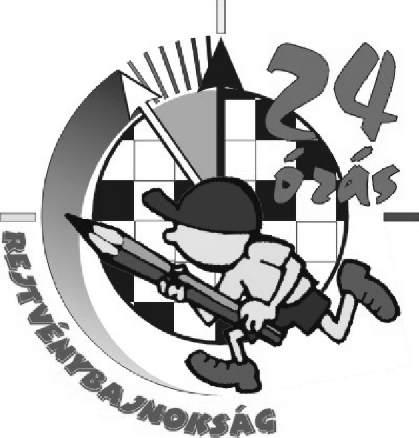
\includegraphics[height=2cm]{24hlogo.jpg}};
    \node[t] at (k) {Puzzles by \\ Robert Vollmert};
\end{tikzpicture}}


\newcommand{\mytitlepage}[1]{%
\begin{center}

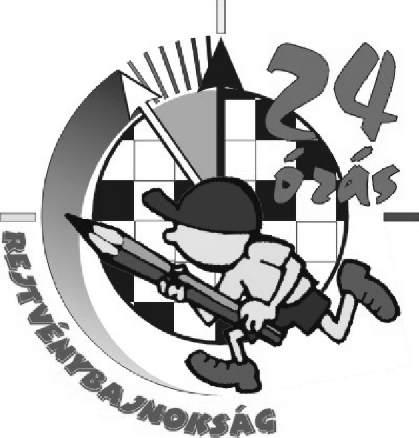
\includegraphics[height=5cm]{24hlogo.jpg}%
\vspace{1cm}%

{\Huge\bfseries 14th 24 Hours Puzzle Championship} \\[2em]
{\Large
   March 21-23, 2014 \\
   Hotel Amadeus \\
   Budapest \\
}%

\vspace{1cm}%

{\Large #1}%

\vspace{1cm}%

{\large\scshape
\begin{tabular}{lr@{ }ll}
LITS & 30 & points & \\
LITS Plus & 145 & points & (15 + 30 + 40 + 60) \\
Geradeweg & 150 & points & (30 + 30 + 30 + 60) \\
Nurikabe & 90 & points & (30 + 60) \\
Latin Tapa & 40 & points & \\
Sudoku & 20 & points & \\
Thermo-Sudoku & 90 & points & \\
Row-Kropki Pyramid & 70 & points & (30 + 40) \\
Slither Link & 30 & points & \\
Liar Slither Link & 90 & points & \\
Tight-Fit Skyscrapers & 20 & points & \\
Double Back & 40 & points & \\
Word Loop & 35 & points & \\
Word Search & 40 & points & \\
Curve Data & 30 & points & \\
Slalom & 30 & points & \\
Compass & 50 & points & (20 + 30) \\
\midrule
{\bfseries Total} & {\bfseries 1000} & {\bfseries points} \\
\end{tabular}
}
\end{center}}%



\renewcommand{\headrulewidth}{0pt}
\fancyhf{}
\lhead{\pageframe}

\begin{document}
\pagestyle{empty}
\ititleframe
\mytitlepage{Solutions to puzzles by Robert Vollmert}

\newpage
\pagestyle{fancy}

\newcommand{\ruleslits}{%
Shade some cells, such that each area has four shaded cells, 
forming a tetromino (four orthogonally connected cells). All
shaded cells must be connected orthogonally, and there can't
be any 2-by-2 square consisting entirely of shaded cells.
Furthermore, no two of the same type of tetromino touch along
an edge. Here, ``same'' is up to rotation and reflection, the
four types are the L, I, T and S tetrominos.}

\newcommand{\ruleslitsplus}{%
Shade some cells, such that the shaded cells within an area,
if any, form a single tetromino (four orthogonally connected cells).
All shaded cells must be connected orthogonally, and there can't
be any 2-by-2 square consisting entirely of shaded or entirely
of unshaded cells.
Furthermore, no two of the same type of tetromino touch along
an edge. Here, ``same'' is up to rotation and reflection, the
four types are the L, I, T and S tetrominos.

\vspace{0.5em}
This differs from standard LITS in that some areas may remain empty, 
and the no-2-by-2 rule also applies to white cells.}

\newcommand{\rulesgeradeweg}{%
Draw a loop that travels horizontally and vertically from cell center
to cell center and that visits each clue, such that the length of
every straight segment that meets a clue is equal to that clue.}

\newcommand{\rulesnurikabe}{%
Shade some cells such that all shaded cells are connected
orthogonally, and there is no 2-by-2 square that consists
entirely of shaded cells.
The shaded cells divide the unshaded cells
into islands of orthogonally connected cells. Each clue
must be part of exactly one island, and the size of that
island must be equal to the clue.}

\newcommand{\ruleslatintapa}{%
Write letters in some cells such that all letter cells
are connected orthogonally, and such that there is no
2-by-2 square of lettered cells. All rows and columns
must contain the same set of letters. Words in clue
cells must be readable clockwise around the clue,
without gaps and separated by non-letter cells. The
clue cells count as non-letter cells.}

\newcommand{\rulessudoku}{%
Place a number from 1 to 9 in each cell, such that
every row, column and outlined 3-by-3 square contains
every number from 1 to 9.}

\newcommand{\rulesthermosudoku}{%
Place a number from 1 to 9 in each cell, such that
every row, column and outlined 3-by-3 square contains
every number from 1 to 9. Numbers along a thermometer
must increase strictly from the bulb.}

\newcommand{\rulesrowkropkipyramid}{%
Place a number from 1 to 9 in each cell, such that for
any two horizontal neighbours, the number between and
above the two is their sum or their difference. In gray
rows, all numbers must be distinct, while in white rows,
there must be at least one pair of duplicate numbers.

\vspace{0.5em}
If an edge between horizontal neighbours is marked with
a white dot, the difference between the two numbers is 1.
If it is marked with a black dot, one number is double the
other number. If there is no mark, neither of the above
conditions apply.}

\newcommand{\rulesslitherlink}{%
Draw a single loop consisting of vertical and horizontal
segments between dots that does not touch or cross itself.
Clue numbers indicate the number of adjacent edges that
are used by the loop.}

\newcommand{\rulesliarslitherlink}{%
Draw a single loop consisting of vertical and horizontal
segments between dots that does not touch or cross itself.
Clue numbers indicate the number of adjacent edges that
are used by the loop, but: In every row and every column,
there is precisely one clue that is incorrect.}

\newcommand{\rulesskyscraperstightfit}{%
Place a number between 1 and 6 (1 and 5 in the example)
in each cell (one in each
triangle for divided cells) such that each row and each
column contains every number. Clues outside the grid
indicate the number of digits that can be seen when looking
into the corresponding row or column. Larger numbers block
the sight to smaller numbers.}

\newcommand{\ruleswordloop}{%
Place each of the given words in the grid vertically,
horizontally or diagonally in any direction, such that
there is at most one letter in each cell, such that all
given letters are used by one of the words, and such
that all words form a single loop, each end of each
word being an end of one other word. Words may intersect
at any point, can touch or use the same letter multiple
times, and adjacent letters are allowed to form
words that aren't part of the loop.}

\newcommand{\ruleswordsearch}{%
Complete the grid by putting letters in the unfilled squares,
and find each of the given terms (without spaces) in the grid.
The terms may read vertically, horizontally or diagonally in any
direction.}

\newcommand{\rulescurvedata}{%
Draw lines that connect cell centers horizontally or
vertically, such that each cell is connected to precisely
one cell with a clue. The shape of lines connected to a
clue must be like the clue in that the relative position
of horizontal and vertical segments and turns must be the
same, without rotations or reflections. The lengths of
straight segments may vary, but must not be 0.}

\newcommand{\rulesdoubleback}{%
Draw a single loop travelling orthogonally from cell centre
to cell centre that visits each cell, and that enters and
exits each area exactly twice each.}

\newcommand{\rulesslalom}{%
Draw a diagonal in each cell such that each clue is equal
to the number of diagonals meeting that vertex, and such
that the diagonals don't enclose any area completely.}

\newcommand{\rulescompass}{%
Split the grid into orthogonally connected regions, one for
each clue. The number at the top of a clue must be equal to
the number of cells within the region that lie above the clue,
regardless of horizontal position. The other numbers work
analogously for cells to the right, below and to the left
of the clue.}


\newcommand{\expl}[1]{\includegraphics[scale=0.5]{../#1.pdf}}

\newcommand{\puzzledef}[3]{%
\noindent{
\centering
\begin{tabularx}{\textwidth}{X c}%
\paragraph{#1}%
#2
&
\raisebox{0pt}{\raisebox{-\height}{\expl{#3}}}%
\end{tabularx}
\\[1ex]
}}%

\newcommand{\puzzledefvert}[4]{%
\noindent\adjustbox{padding=1.5ex}{%
\begin{minipage}{#4}
\paragraph{#1}%
#2
\\[1ex]
\begin{center}
\expl{#3}%
\end{center}
\end{minipage}
}}%

\newcommand{\puzzleat}[3]{%
\begin{tikzpicture}[remember picture, overlay, shift={(dA)}]
%   \draw (0,0) grid (22,30);
   \node[inner sep=0] at #2 (x) {\includegraphics[trim=0.2cm 0.2cm 0.2cm 0.2cm]{../#1-sol.pdf}};
   \node[yshift=0.25cm, anchor=south east] at (x.north east) {\Large #3};
%   \node[xshift=0.25cm, anchor=north west] at (x.north east) {\Large #3};
\end{tikzpicture}}%

\newcommand{\puzzle}[2]{%
\begin{tikzpicture}
   \node[inner sep=0] (x) {\includegraphics[trim=0.2cm 0.2cm 0.2cm 0.2cm]{../#1-sol.pdf}};
   \node[yshift=0.25cm, anchor=south east] at (x.north east) {\Large #2};
\end{tikzpicture}}%

\newcommand{\puzzler}[2]{%
\begin{tikzpicture}
   \node[inner sep=0] (x) {\includegraphics[trim=0.2cm 0.2cm 0.2cm 0.2cm]{../#1-sol.pdf}};
   \node[xshift=0.25cm, anchor=north west] at (x.north east) {\Large #2};
\end{tikzpicture}}%

\newcommand{\puzzlec}[2]{%
\begin{center}
\puzzle{#1}{#2}
\end{center}}

\newcommand{\puzzlerc}[2]{%
\begin{center}
\puzzler{#1}{#2}
\end{center}}

\puzzleat{lits-1}{(13,16.5)}{30}
\puzzleat{litsplus-easy-growing}{(13,6)}{15}

\puzzledefvert{LITS}{\ruleslits}{lits-example}{0.35\textwidth}

\vspace{3cm}
\puzzledefvert{LITS+}{\ruleslitsplus}{litsplus-example}{0.35\textwidth}

\newpage

\puzzleat{litsplus-x}{(4,18.2)}{30}
\puzzleat{litsplus-snakes}{(13.5,17)}{40}
\puzzleat{litsplus-3x5}{(13.1,5.5)}{60}

\vspace{10cm}
\puzzledefvert{LITS+}{\ruleslitsplus}{litsplus-example}{0.35\textwidth}

\newpage
\puzzledef{Geradeweg}{\rulesgeradeweg}{geradeweg-example}

\puzzleat{geradeweg-anti}{(5,4.5)}{30}
\puzzleat{twin-gn-geradeweg}{(13.5,4.5)}{30}
\puzzlec{geradeweg-pyramids}{30}

\newpage

\puzzledef{Geradeweg}{\rulesgeradeweg}{geradeweg-example}

\vspace{3cm}
\puzzlec{geradeweg-24}{60}

\newpage
\puzzledef{Nurikabe}{\rulesnurikabe}{nurikabe-example}

\puzzlec{twin-gn-nurikabe}{30}
\puzzlec{nurikabe1}{60}

\newpage
\puzzledef{Latin Tapa}{\ruleslatintapa}{latintapa-example}

\vspace{3cm}
\puzzlec{latintapa}{40}

\newpage
\puzzleat{sudoku-2}{(13.5,17)}{20}
\puzzleat{sudoku-thermo-cva-easier}{(13.5,5.5)}{90}

\vspace{2cm}
\puzzledefvert{Sudoku}{\rulessudoku}{sudoku-example}{0.35\textwidth}

\vspace{6cm}
\puzzledefvert{Thermo-Sudoku}{\rulesthermosudoku}{sudoku-thermo-example}{0.35\textwidth}

\newpage
\puzzledef{Row-Kropki Pyramid}{\rulesrowkropkipyramid}{pyramid-kropki-example}

\vspace{1cm}
\puzzlec{pyramid-kropki-1}{30}

\vspace{1cm}
\puzzlec{pyramid-kropki-2}{40}

\newpage

\puzzleat{slither-easy}{(13.5,17)}{30}
\puzzleat{slither-liar}{(13.5,5.5)}{90}

\vspace{1cm}
\puzzledefvert{Slither Link}{\rulesslitherlink}{slitherlink-example}{0.35\textwidth}

\vspace{5.5cm}
\puzzledefvert{Liar Slither Link}{\rulesliarslitherlink}{slitherlink-liar-example}{0.35\textwidth}

\newpage
\puzzledefvert{Tight-Fit Skyscrapers}{\rulesskyscraperstightfit}{skyscraper-tightfit-example}{0.35\textwidth}
\puzzleat{skyscraper-tightfit}{(13.5,19)}{20}

\puzzledef{Double Back}{\rulesdoubleback}{doubleback-example}
\puzzlerc{doubleback-S}{40}

\newpage
\puzzledef{Word Loop}{\ruleswordloop}{wordloop-example}

\vspace{3cm}
\puzzlec{wordloop-colors}{35}

\newpage
\puzzledef{Word Search}{\ruleswordsearch}{wordsearch-example}

\vspace{3cm}
\puzzlec{wordsearch-crawlgods}{40}

\newpage
\puzzleat{curvedata-pento}{(13.5,17)}{30}
\puzzleat{slalom3}{(13.5,6)}{30}

\vspace{1.5cm}
\puzzledefvert{Curve Data}{\rulescurvedata}{curvedata-example}{0.35\textwidth}

\vspace{4.5cm}
\puzzledefvert{Slalom}{\rulesslalom}{slalom-example}{0.35\textwidth}




\newpage
\puzzledef{Compass}{\rulescompass}{compass-example}

\puzzlec{compass-easy}{20}

\vspace{1ex}
\puzzlec{compass-12}{30}

\end{document}
